\section{Software Entwicklung}
Die Softwareentwicklung ist schwierig,Hauptgrund: Komplexität.  
Ein Softwareprojekt kann sich aufgrund der Komplexität in ein Werwolf verwandeln. Dieser kann nur mit einer Silberkugel getötet werden.\\
Frederic Brooks hat dies analysiert. 
\begin{itemize}
	\item \textit{"No Silver Bullet"} $\rightarrow$ Es gibt kein Wundermittel um komplexe Software zu entwickeln
	\item \textit{"{}Adding Manpower to a late Software project makes it later"} $\rightarrow$ Neue Leute müssen sich einarbeiten und Kommunikationsaufwand steigt. 
\end{itemize}

\subsection{Schwierigkeiten}
2 Arten von Schwierigkeiten führen zu Komplexität
\begin{table}[h]
	\begin{tabular}{|l|l|}
	\hline
	\textbf{Essentielle Schwierigkeiten}  & \begin{tabular}[c]{@{}l@{}}Verursacht durch Komplexität des Problems\\ Essenz: Kern der Sache\end{tabular}                \\ \hline
	\textbf{Akzidentelle Schwierigkeiten} & \begin{tabular}[c]{@{}l@{}}Selbst verursacht durch falsche Methoden, Mittel\\ Akzidenz: Art der Realisierung\end{tabular} \\ \hline
	\end{tabular}
\end{table}

\subsection{Bewältigung der Komplexität}	
		\begin{enumerate}
			\item Teile und herrsche \textit{"divide et impera"}
					\begin{itemize}
						\item Problem in Teilprobleme aufteilen
						\item Jedes Teilproblem für sich alleine lösen, alle zusammen ergeben Problemlösung
						\item Möglichst eigenständige Teile (hohe Kohäsion)
						\item Möglichst geringe Abhängigkeiten (kleine Kopplung)
					\end{itemize}
			\item Abstraktion
					\begin{itemize}
						\item Definition: Weglassen von Aspekten, die für den gegenwärtigen Zweck nicht wichtig sind.
					\end{itemize}
			\item Modelle
					\begin{itemize}
						\item Abstraktion der realen Welt, Es gibt zwei Typen von Modellen:
                        \begin{itemize}
                        \item Design-Modelle (Lösungsdarstellung)
                        \item Domain-Modelle (Problemdarstellung)
                        \end{itemize}
					\end{itemize}
		\end{enumerate}

\subsection{Vorgehen zur Softwareentwicklung}
	\begin{enumerate}
		\item Analyse
			\begin{itemize}
				\item Ziel: Man weiss mehr als vorher, Man weiss WAS entwickelt werden soll.
				\item Probleme, Ideen, Anforderungen aufnehmen
				\item Erstellen eines Pflichtenhefts
				\item \textit{"doing the right things"} $\rightarrow$ Die richtigen Dinge tun
			\end{itemize}
		\item Design
			\begin{itemize}
				\item Ziel: Man weiss WIE das Produkt entwickelt werden soll
				\item Erstellen eines Grobentwurfs und eines Detailentwurfs. Es entsteht noch kein Code. Nur Baupläne für die Software
				\item \textit{"doing things right"} $\rightarrow$ Die Dinge richtig tun
			\end{itemize}
		\item Implementierung
			\begin{itemize}
				\item Entwicklung des Sourcecodes 
			\end{itemize}
		\item Test 
	\end{enumerate}
\pagebreak

\subsection{Vorgehensmodelle (Klassisch)}
\subsubsection{Begriffe}
\begin{itemize}
	\item Ein Vorgehensmodell dient dazu die Softwareentwicklung übersichtlicher zu gestalten
	\item Schwergewichtiger Prozess $\rightarrow$ Klassische Softwareentwicklung
	\item Leichtgewichtiger Prozess $\rightarrow$ Agile Softwareentwicklung
	\item Big-Bang $\rightarrow$ Software wird Kunden fertig entwickelt präsentiert. Gefahr ist gross, dass der Kunde sich die Software anders vorgestellt hat. Folge: Vertrauen des Kunden wird zerstört und hektisches Nachbessern wird nötig. 
\end{itemize}

\subsubsection{Wasserfall-Modell}
\begin{minipage}{10cm}
	\begin{itemize}
		\item linear
		\item nicht iterativ
		\item in Realität nicht durchführbar
		\item Freigabe beim Abschluss jeder Phase
		\item Es gibt kein zurück, alles muss beim ersten Mal richtig gemacht werden. 
	\end{itemize}
\end{minipage}
\begin{minipage}{5cm}
	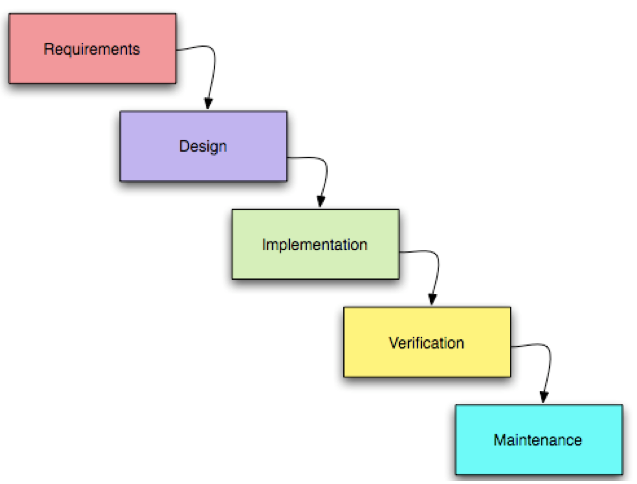
\includegraphics[width=5cm]{images/wasserfall_modell.png}
\end{minipage}
	
\subsubsection{Kaskade}
	\begin{minipage}{10cm}
		\begin{itemize}
			\item Erweiterung des Wasserfalls um Korrekturschleifen
			\item In Realität durchführbar
			\item Man kann immer nur eine Phase zurück
		\end{itemize}
	\end{minipage}
	\begin{minipage}{5cm}
	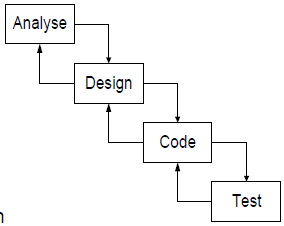
\includegraphics[width=5cm]{images/kaskade.png}	
	\end{minipage}

\subsubsection{V-Modell}
\begin{minipage}{8cm}
	\begin{itemize}
		\item Korrespondierende Tests
		\item x-Achse = Zeit
		\item y-Achse = Detaillierungsgrad
		\item Weiterentwicklung V-Modell XT,\newline
        immer projektspezifische Anpassungen nötig\newline
        (XT = Extreme Tailoring, engl. „to tailor“ = schneidern)
	\end{itemize}
\end{minipage}
\begin{minipage}{9cm}
	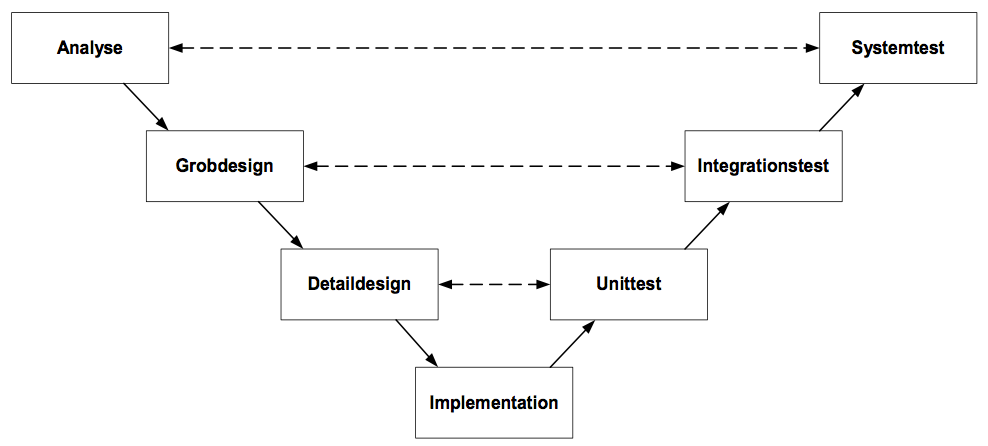
\includegraphics[width=9cm]{images/v_modell.png}	
\end{minipage}


\subsubsection{Iterative / Inkrementelle Entwicklung / Spiralmodell}
\begin{minipage}{8cm}
Es gibt zwei Modelle: Das Spiralmodell und RUP (Rational Unified Process).\\
\\
	\textbf{Inkrementell:}
		\begin{itemize}
			\item Resultat in Schritten entwickeln
			\item Jeder Schritt ist Teil des Endresultats
		\end{itemize}
	\textbf{Iterativ:}
		\begin{itemize}					
			\item Erste Version entwickeln
			\item In weiteren Schritten bessere Versionen erstellen
		\end{itemize}
\end{minipage}
\begin{minipage}{6cm} %TODO Grafik grösser
	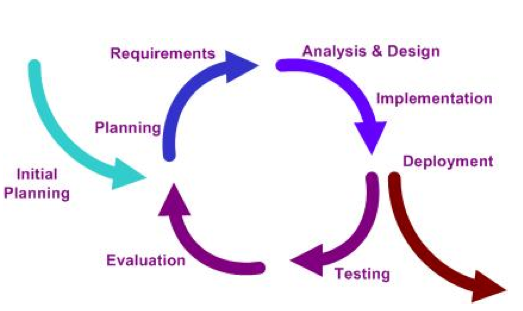
\includegraphics[width=5cm]{images/iterative_entwicklung.png}
\end{minipage}
\begin{minipage}{8cm}
	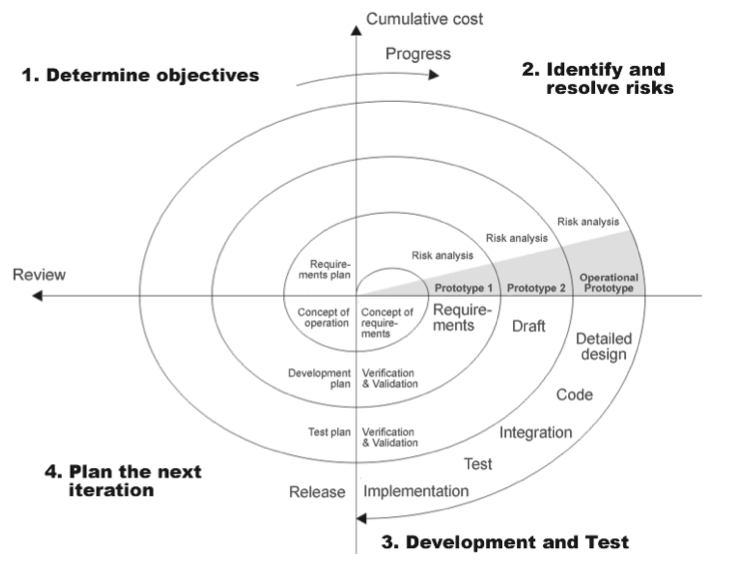
\includegraphics[width=5cm]{images/spiral_modell.png}
\end{minipage}


\subsection{Vorgehensmodell (Agil)}
\begin{itemize}
	\item weniger formalisiert als schwerfällige, bürokratische klassische Softwareentwicklung
	\item agil = flink, beweglich
	\item Individuen und Interaktionen gelten mehr als Prozesse
\end{itemize}

Agile Softwareentwicklung besteht aus:
\begin{enumerate}
	\item \textbf{Agile Werte:} bilden das Fundament.
	\item \textbf{Agile Prinzipien:} sind Handlungsgrundsätze, die auf agilen Werten basieren.
	\item \textbf{Agile Methoden:} sind konkrete Verfahren, die sich auf agile Werte und Prinzipien stützen.
	\item \textbf{Agile Prozesse:} sind die Zusammenfassungen agiler Methoden.
	\\ 
\end{enumerate}

\begin{multicols}{2}
\subsubsection{XP (Extreme Programming)}
\begin{minipage}{10cm}
	\begin{itemize}
		\item Bekanntester agiler Prozess
	\end{itemize}
\end{minipage}
\begin{minipage}{5cm} %TODO Besser auflösung
	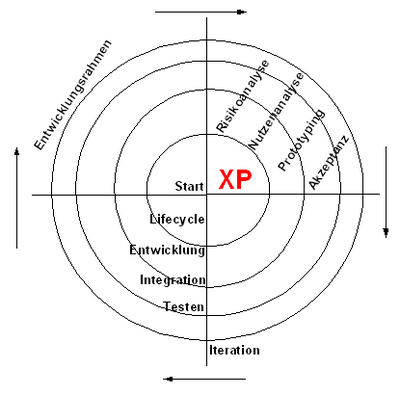
\includegraphics[width=7cm]{images/extreme_programming.png}
\end{minipage}

\subsubsection{Scrum} %TODO Scrum weiter nach links Bild grösser
\begin{minipage}[l]{10cm}
	\begin{itemize}
		\item Gedränge
		\item Basis: Sprints von 15-30 Tagen wo neuer Software-Release erstellt wird
	\end{itemize}
\end{minipage}
\begin{minipage}{7cm}
	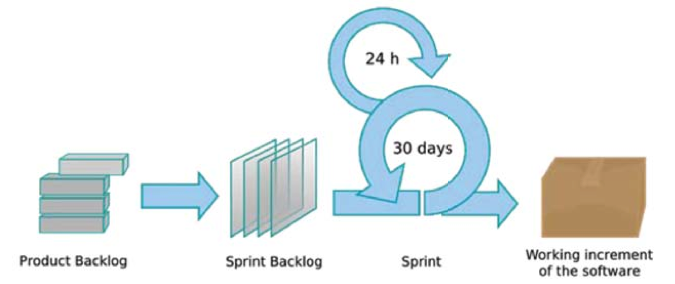
\includegraphics[width=8cm]{images/scrum.png}
\end{minipage}
\\
\end{multicols}

\subsection{Objektorientierte Softwareentwicklung (OOAD)}
\begin{minipage}{13cm}
	\begin{itemize}
		\item Modelle auf allen Stufen: OO-Analyse $\rightarrow$ OO-Design $\rightarrow$ OO-Implementation
		\item Objekte sind Abstraktionen von realen Dingen
		\item Klassen entstehen durch Gruppieren und Zusammfassen von Objekten mit gleicher Datenstruktur
		\item Gleiche Notation bei OOA, OOD, OOI
		\item Darstellung mit UML
		\item OOAD kann in jedem Vorgehensmodell verwendet werden
	\end{itemize}
\end{minipage}
\begin{minipage}{6cm}%TODO anderes UML
	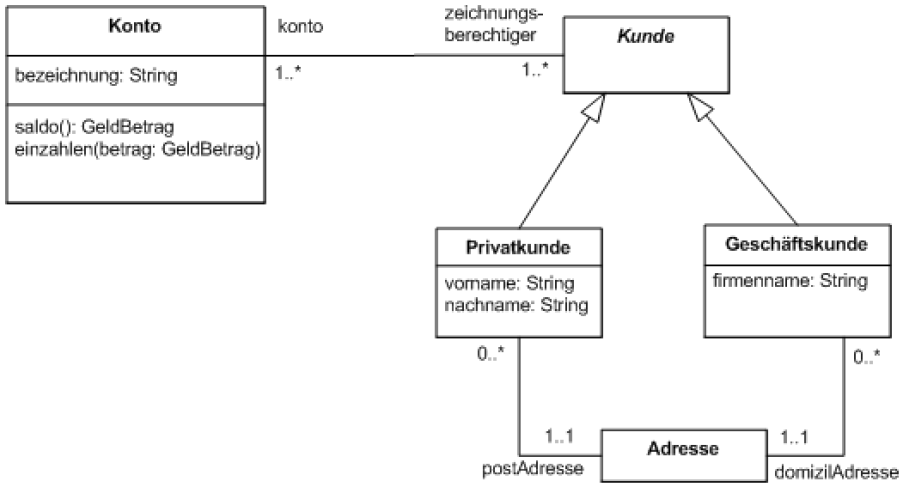
\includegraphics[width=6cm]{images/uml.png}
\end{minipage}

\subsection{Kriterien für die Wahl des Modells}
\begin{itemize}
	\item Verfügbarkeit der Ressourcen
	\item Projektkomplexität
	\item Zeitpunkt von Änderungen (diskret, laufend)
	\item Qualität der Anforderungsdefinitionen
	\item Stabilität bzw. Volatilität der Anforderungen
\end{itemize}